\chapter{RailLab: A Desktop Research Console}
\label{ch:raillab}

\Cref{ch:refsim} built the reference simulator and \cref{ch:routes} built the pipeline that feeds it real terrain. Both are libraries: they are driven from notebooks and scripts, and everything they need, a consist, a route, a set of driving commands, arrives as Python objects assembled by hand. That is a workable way to produce a figure for a chapter. It is a poor way to explore, and exploration is most of what the work in the following chapters actually consists of.

This chapter documents \emph{RailLab}, a desktop application built over the same backend. It is not a deliverable of the thesis in its own right, and none of the numerical claims in later chapters depend on it. It is a research instrument, and it is documented here for the same reason the simulator's staging is documented: the way a tool shapes what questions get asked is part of the method.

\section{Why a graphical console}
\label{sec:raillab_motivation}

Three problems motivated building it.

The first is the cost of a question. Asking ``what happens to coupler forces if this train is thirty cars longer on this particular grade'' requires, in script form, editing a consist definition, re-resolving car parameters, rebuilding a scenario, re-running the solver, and re-plotting, with the answer arriving a few minutes and several opportunities for error later. Most such questions are never asked, not because they are uninteresting but because the friction exceeds the curiosity. Collapsing that loop to a dropdown and a button changes which questions get asked at all.

The second is the gap between a number and a shape. A simulator returns arrays. The failure modes that matter here, a run-in that the coupler model resolves unphysically, a grade artifact surviving the smoothing stage in \cref{ch:routes}, a control profile whose brake command overlaps traction in a way no operator would produce, are visible immediately in a plot and nearly invisible in a summary statistic. Later chapters lean on trip-level error metrics; those metrics are trustworthy only in proportion to how much of the underlying trajectory behavior has been looked at directly.

The third is reproducible bookkeeping. The experiments in later chapters need many consists run against comparatively few routes, and every artifact involved, a car type, a train, a control profile, a route, has to be nameable, saveable, and reloadable so that a run can be repeated exactly. Building an interface around those artifacts forced them to become first-class, serializable objects in the backend rather than variables in a notebook cell, which is a benefit the headless path inherits.

\section{Architecture}
\label{sec:raillab_architecture}

The governing constraint is that the user interface never imports the numerical stack. The backend packages, \texttt{simulator2} and \texttt{routegen}, are unchanged by the application's existence; the application reaches them only through a thin service layer. \Cref{fig:raillab_stack} summarizes the arrangement.

\begin{figure}[htbp]
\centering
\caption{RailLab's layering. Screens call services; services are the only modules that import the numerical backend, and they return plain data. The backend packages are unchanged by the application's existence and continue to run headless.}
\label{fig:raillab_stack}
\end{figure}

The layering has three consequences that matter more than the tidiness. The backend still runs headless, so notebooks, the batch dataset generator, and the figures in this document have no dependency on the interface toolkit. The services contain no interface code at all, so each is unit-testable without a display. And the boundary is a natural insertion point: the surrogate model and the controller developed in later chapters attach as additional services without any existing screen changing.

Within the application, each screen owns one stage of the workflow and communicates through shared service objects rather than by reaching into its neighbors. The \textsc{consist} and \textsc{simulate} screens share one consist service, so a train edited on one appears immediately on the other; \textsc{controls} and \textsc{simulate} likewise share a control-profile service. Signals from a finished run are fanned out by the window shell to the \textsc{results} screen and the status indicator, so neither screen holds a reference to the other.

Long solver calls run off the interface thread. Pressing \textsc{go} constructs a scenario, hands it to a worker object moved onto a dedicated thread, and returns immediately; the worker emits either a result or an error message when the integration finishes. Because the reference simulator integrates the whole time span in one adaptive solver call, there is no intermediate hook to report progress against or to interrupt, and the stop control is correspondingly disabled. This is a real limitation rather than an oversight: interrupting or streaming a run requires a stepwise integrator, which the reference implementation deliberately does not use.

\section{The workflow, screen by screen}
\label{sec:raillab_screens}

\subsection{Route}

The route screen browses the output of \cref{ch:routes}. Each processed route is listed, and selecting one loads its per-vertex arrays and renders three chainage-linked plots, elevation, grade, and curvature, alongside a summary panel: length, vertex count, elevation range, total climb and descent, grade range, maximum curvature and the corresponding minimum radius, speed-limit range, and the fraction of the line for which the map actually supplied a speed limit. Routes lacking the compact array file the simulator consumes are listed but marked, and the simulate screen will not offer them.

That last field, speed-limit coverage, is the reason the panel exists in this form. It is a data-quality property, not a physical one, and it is exactly the sort of thing that is easy to forget when a route is loaded programmatically and impossible to overlook when it is printed next to the grade range every time the route is opened.

\subsection{Consist}

The consist screen is where trains are assembled, and it implements the three-way split the data model was designed around: a library of reusable car types, an ordered train under construction, and a shelf of saved trains (\cref{fig:raillab_consist}).

A car type is a named template, a locomotive, a loaded grain hopper, a full water tank car, carrying mass split into tare and lading, Davis resistance coefficients, traction and braking ceilings, physical length, and a coupler type. Types are stored one per file as plain text records, so the library is inspectable and version-controllable outside the application. A train is an ordered list of references to those types, which means a train file stays small regardless of length and a correction to a car type propagates to every train that uses it.

Per-car overrides are the escape hatch. Any individual car in a train may override selected fields of its type, tare mass, lading, any Davis coefficient, either force ceiling, while inheriting the rest. This makes ``the same train but with one unusually heavy car'' expressible without polluting the library with a near-duplicate type. A running summary along the bottom reports car count, total mass, total length, and how many vehicles are powered.

\begin{figure}[htbp]
    \centering
    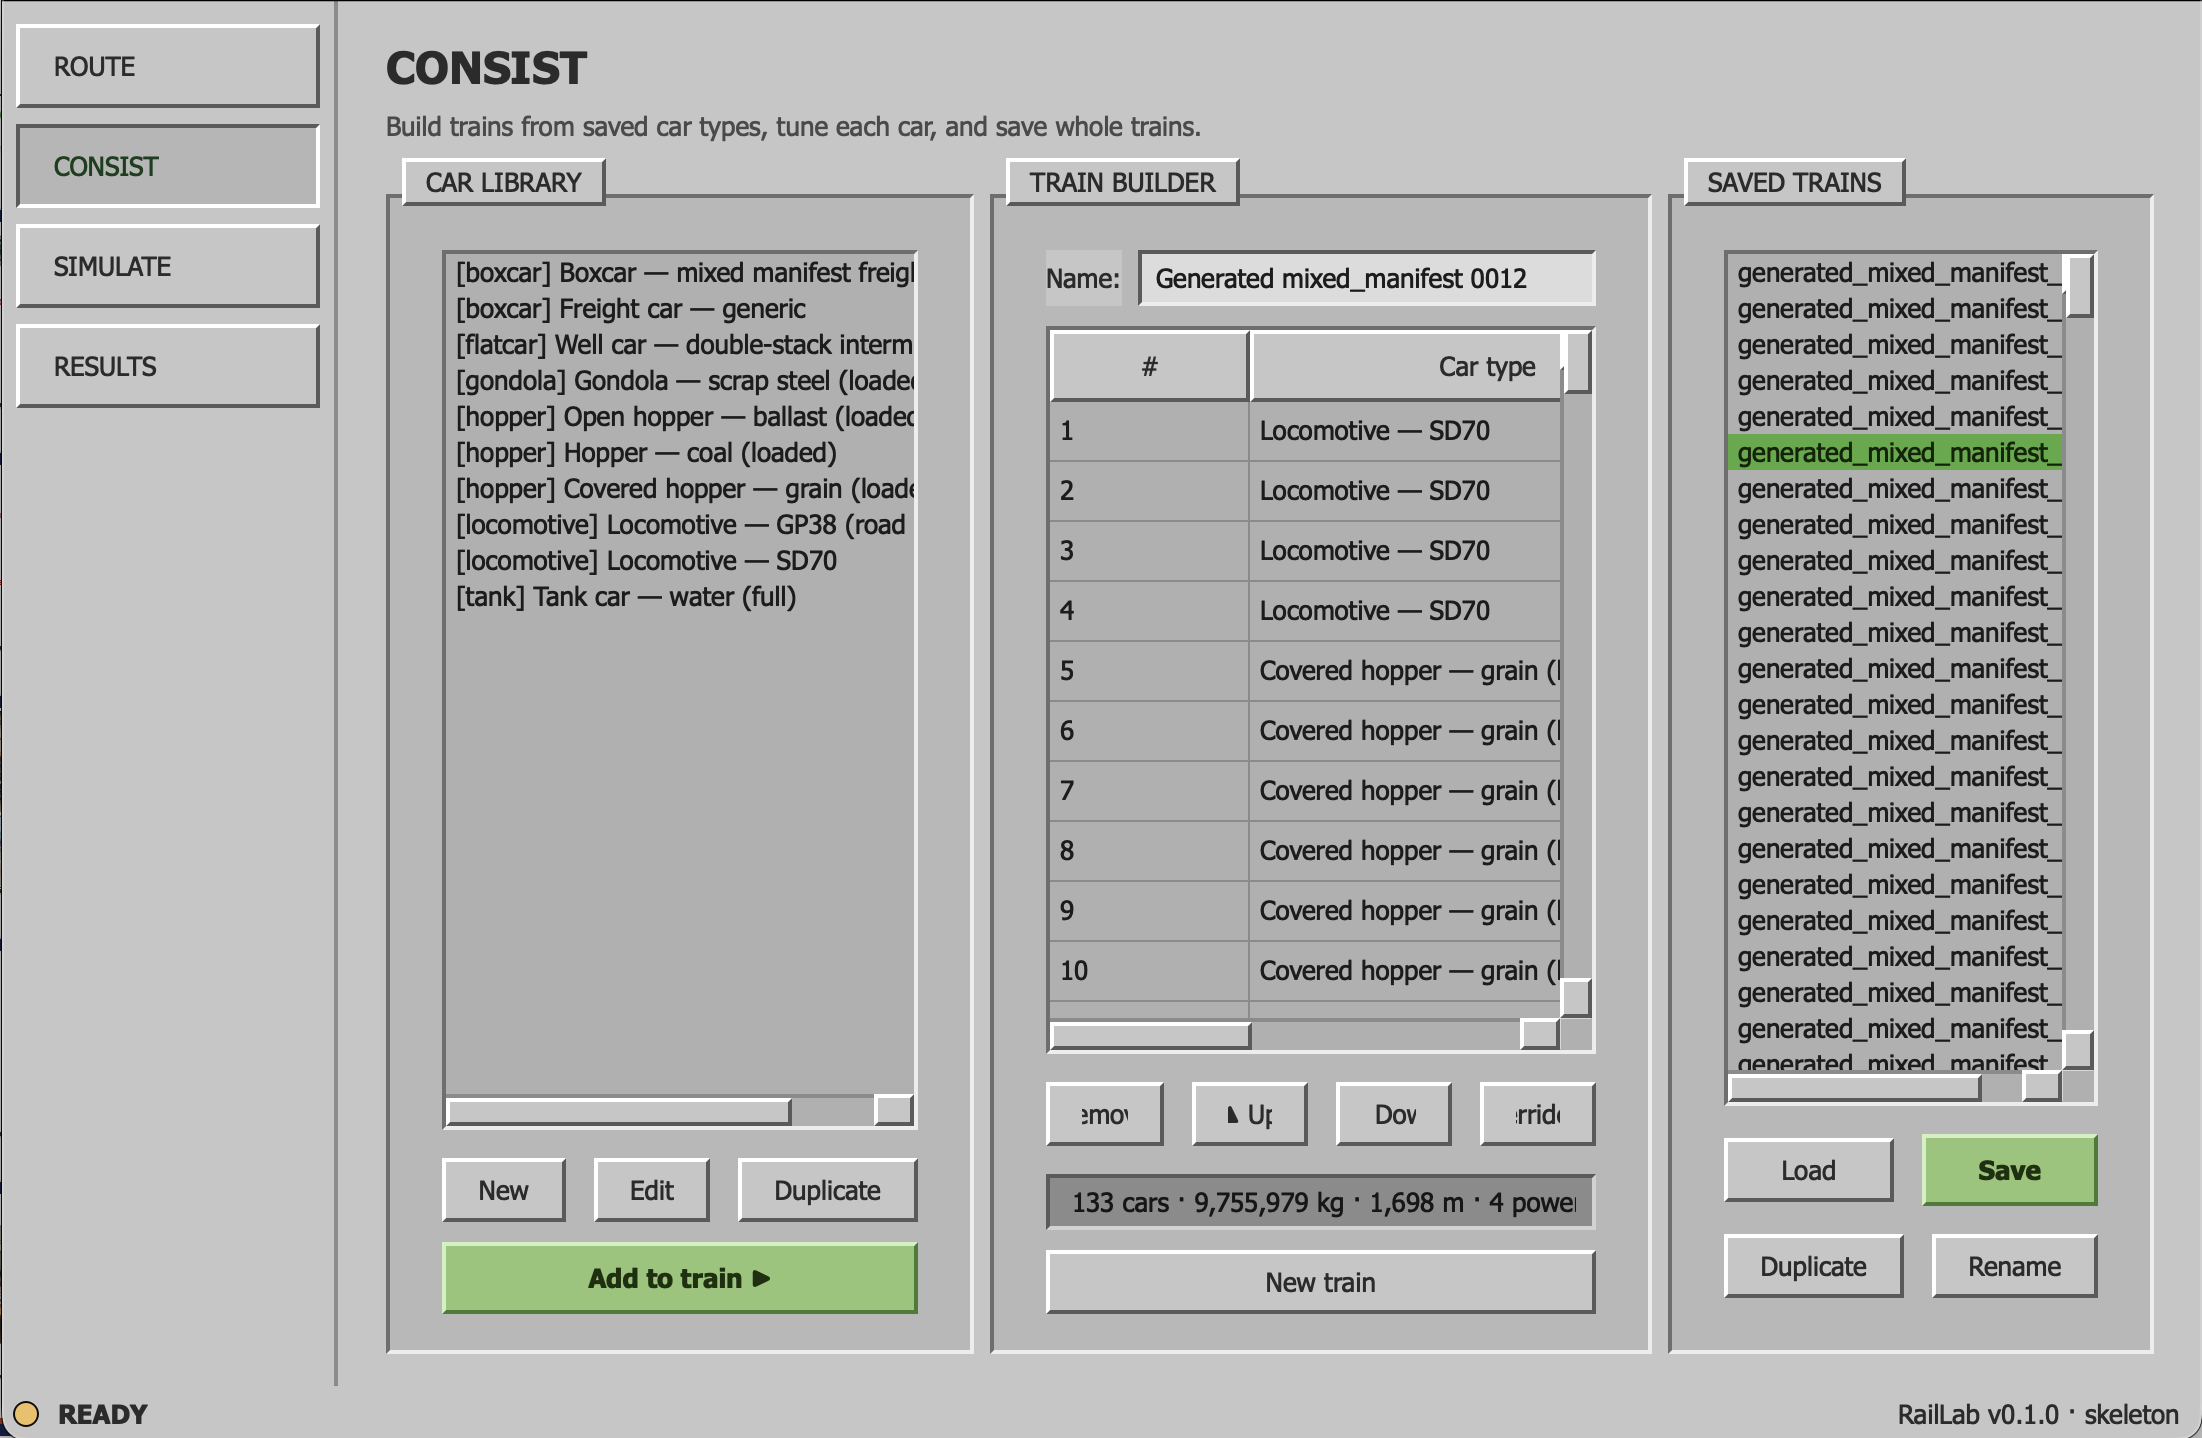
\includegraphics[width=0.92\textwidth]{thesis_imgs_7_15/raillab/raillab_consist.png}
    \caption{The \textsc{consist} screen: a library of reusable car types (left), the ordered train under construction with per-car overrides (centre), and saved trains (right). The running summary reports car count, total mass, total length, and the number of powered vehicles.}
    \label{fig:raillab_consist}
\end{figure}

\Cref{fig:raillab_consist} shows a consist produced by the procedural generator rather than assembled by hand: a mixed-manifest train of 133 cars, roughly 9,756 tonnes, 1698 metres long, with four powered units at the head. The generator writes through the same save path the interface uses, so generated and hand-built trains are indistinguishable downstream, which is what makes the large training sweeps of later chapters possible without a second code path.

\subsection{Controls}

The controls screen generates the driving commands. A control profile is a train-agnostic recipe: piecewise command curves expressed as a \emph{fraction} of each vehicle's own force ceiling rather than in newtons, so one profile drives any consist. Curves are defined by knots and interpolated with the same smoothstep shape the simulator's traction ramp uses, which keeps commands continuous and avoids the stiffness that instantaneous steps introduce.

Profiles are generated randomly under user-specified bounds: duration, number of knots per curve, traction and brake fraction ranges, and the treatment of distributed power (\cref{fig:raillab_controls}). Distributed power units are addressed by role, head-end, mid-train, and rear helper, resolved from each car's label, and may be driven synchronously with a configurable lag behind the head end, independently, or not at all. The preview plots the resulting traction command for each role and the brake command below it; the visible role-to-role offset in the figure is the lag. Generation is seeded, so a profile is reproducible from its configuration alone.

\begin{figure}[htbp]
    \centering
    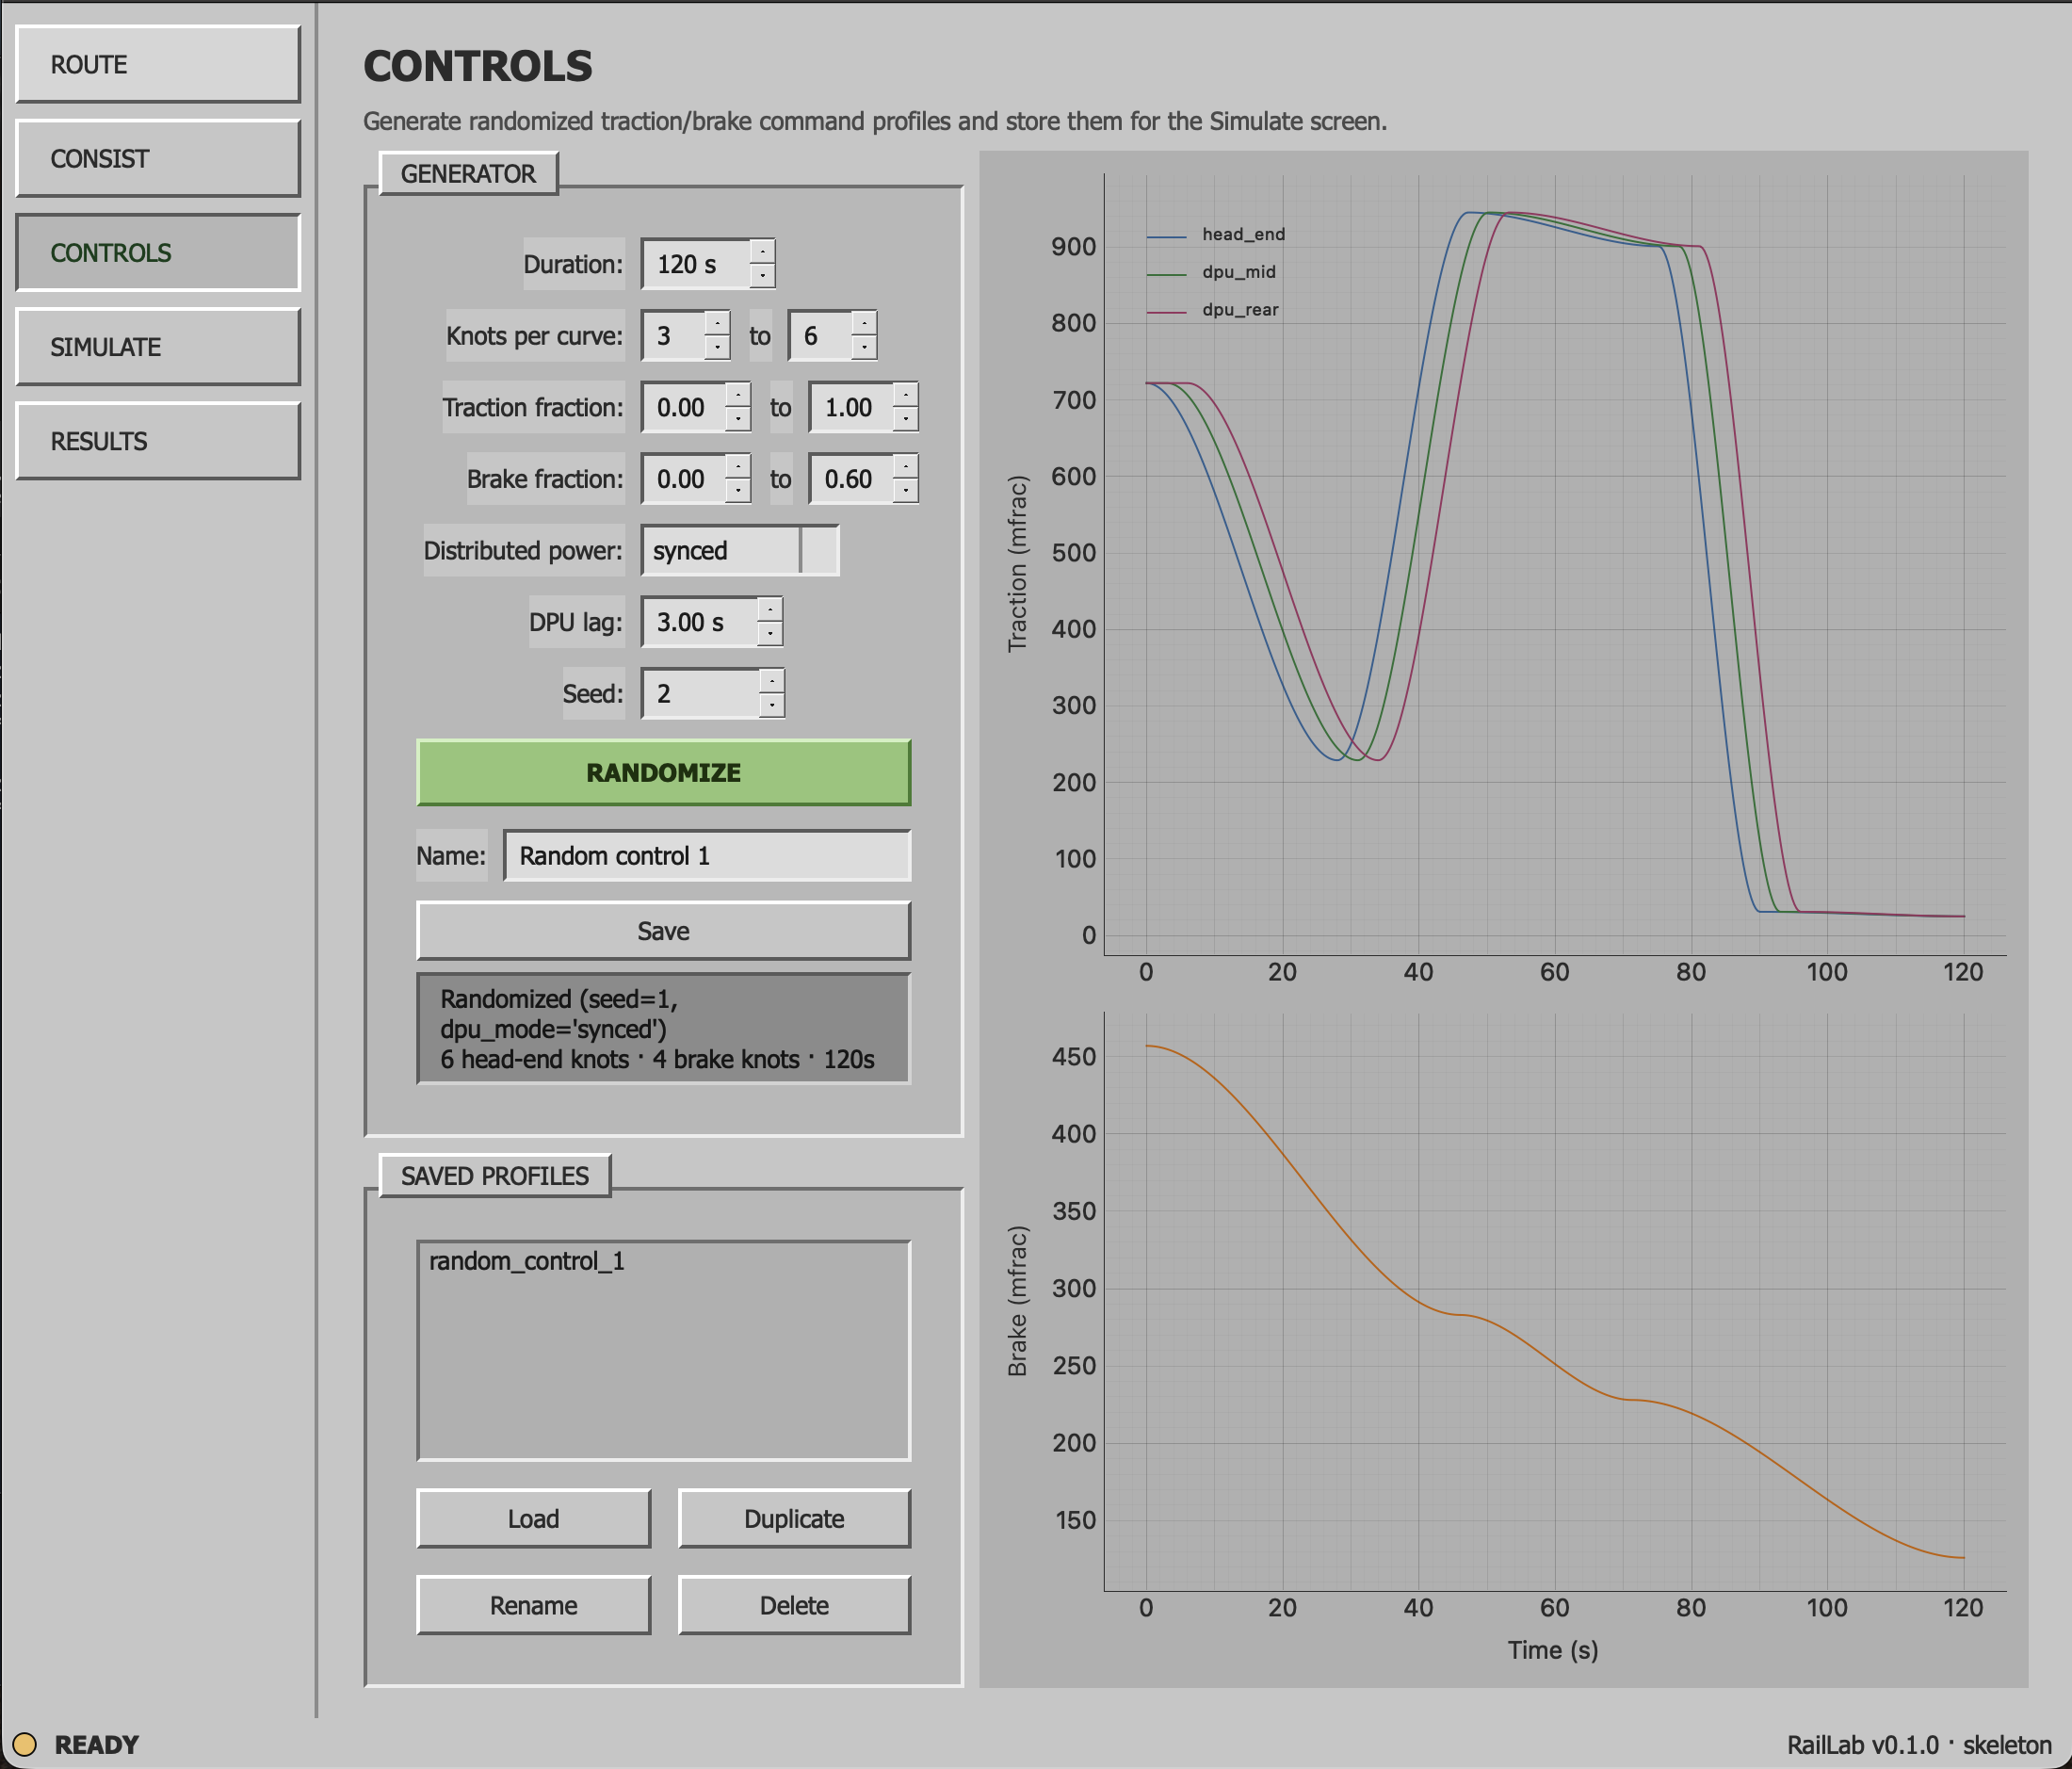
\includegraphics[width=0.92\textwidth]{thesis_imgs_7_15/raillab/raillab_controls.png}
    \caption{The \textsc{controls} screen: randomization bounds and distributed-power settings on the left, with a live preview of the generated traction command per power role (top right) and the shared brake command (bottom right). The offset between the three traction traces is the configured lag of the mid-train and rear helper units behind the head end.}
    \label{fig:raillab_controls}
\end{figure}

Randomized commands are what the surrogate's training set needs: a model trained only on hand-designed, sensible driving would never see the transients that make coupler dynamics hard. The bounded ranges keep the randomness within a plausible envelope rather than making it arbitrary.

\subsection{Simulate and Results}

The simulate screen is deliberately spare. It selects a saved train and a route, sets duration, an optional traction ceiling override, and the curvature-term scale, picks a control profile or falls back to the default ramp, and runs. Everything it needs has already been named and saved elsewhere, which is the point: a run is fully specified by a short list of named artifacts and four numbers, and is therefore trivially repeatable.

Results are plotted as they arrive: every vehicle's speed on one axis and every coupler's force on a second, time-linked axis below it (\cref{fig:raillab_results}). Plotting every vehicle rather than a summary is intentional. The figure shows a 126-vehicle consist over 120 seconds under a randomized control profile, and the structure that carries the information is the \emph{spread} between vehicles: the envelope of the speed traces widening and collapsing as slack runs in and out, and the corresponding fan of coupler forces. Neither is visible in a mean, and the qualitative behavior, oscillation that decays rather than growing, forces that stay bounded, is the sanity check that a summary statistic cannot provide.

\begin{figure}[htbp]
    \centering
    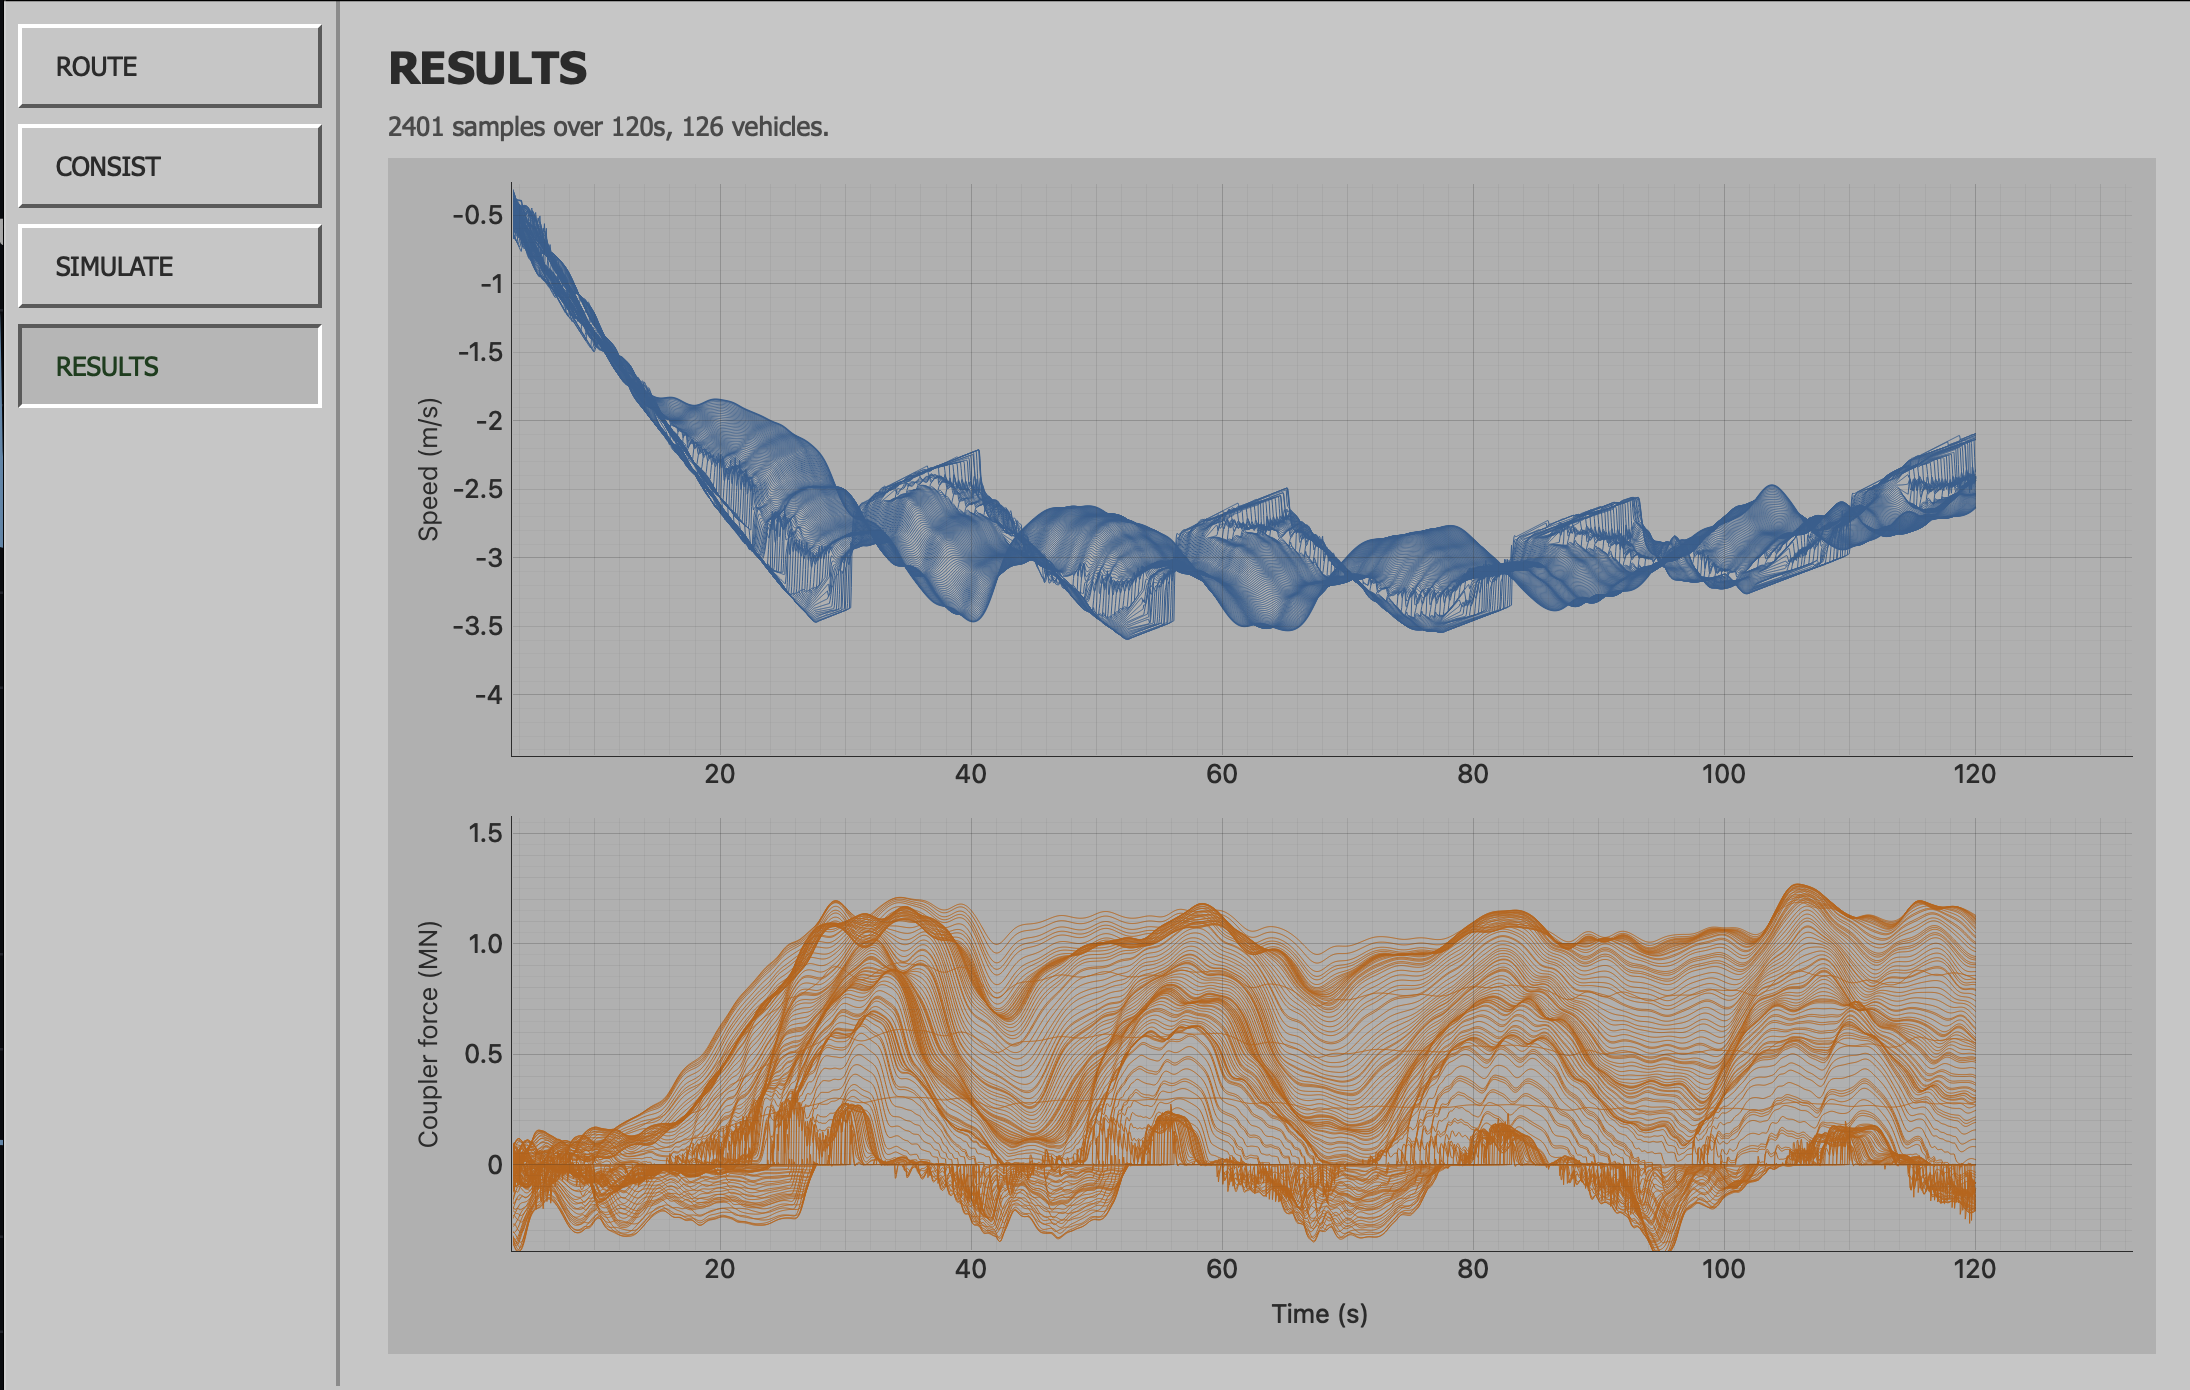
\includegraphics[width=0.92\textwidth]{thesis_imgs_7_15/raillab/sim_results.png}
    \caption{The \textsc{results} screen after a 120\,s run of a 126-vehicle consist under a randomized control profile. Every vehicle's speed is plotted above every coupler's force, on time-linked axes. The information is carried by the spread between traces: the widening and collapsing speed envelope is slack running in and out, with the corresponding fan of coupler forces below.}
    \label{fig:raillab_results}
\end{figure}

\section{Status and limitations}
\label{sec:raillab_status}

RailLab is a working instrument, not finished software, and several limitations bear on how it should be read.

Runs cannot be interrupted or monitored mid-flight, for the reason given in \cref{sec:raillab_architecture}: the solver call is atomic. Long runs therefore occupy the application until they complete, though not the interface thread. The results screen plots the two channels that matter most for the present work and does not yet expose the full node and edge state, nor does it export a run directly; dataset generation remains the job of the headless batch path, which is the correct division, since the interface is for looking at one run and the batch runner is for producing thousands.

Most importantly, nothing in this chapter changes the standing caveat from \cref{ch:refsim}: the parameters in the car library are realistic in shape but are not calibrated to any specific real rolling stock. The application makes it easy to build a train and watch it behave, and that ease should not be mistaken for validation. What is being explored is the reference simulator's behavior, which is exactly what the surrogate of the following chapters is trained to reproduce.

\section{Chapter summary}

This chapter documented RailLab, the desktop console built over the reference simulator and route pipeline. Its architecture keeps the interface strictly separated from the numerical backend through a service layer, so the backend remains headless and testable and later components attach without disturbing existing screens. Its five screens follow the workflow the thesis needs: inspect a route, assemble a consist from a reusable car library, generate randomized driving commands, run, and look at the result. The artifacts it manipulates, car types, trains, control profiles, routes, are the same named, serializable objects the headless batch tooling uses, so interactive exploration and large-scale dataset generation share one representation. \Cref{ch:gpu_dataset} uses that representation to generate the training data at scale.
